% Created by tikzDevice version 0.10.1 on 2018-06-27 15:03:08
% !TEX encoding = UTF-8 Unicode
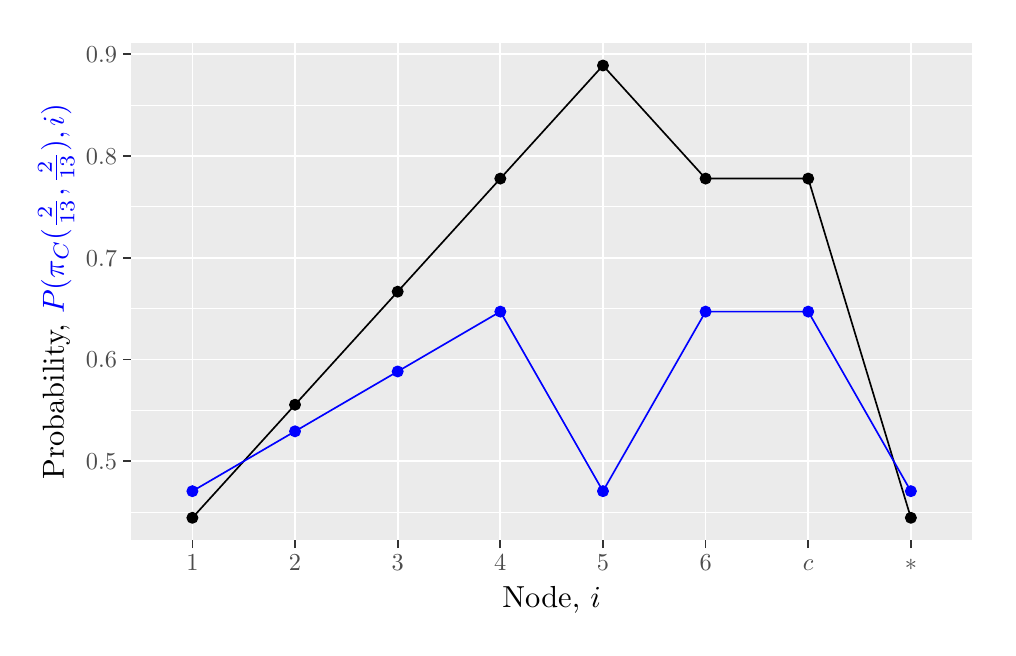
\begin{tikzpicture}[x=1pt,y=1pt]
\definecolor{fillColor}{RGB}{255,255,255}
\path[use as bounding box,fill=fillColor,fill opacity=0.00] (0,0) rectangle (346.90,216.81);
\begin{scope}
\path[clip] (  0.00,  0.00) rectangle (346.90,216.81);
\definecolor{drawColor}{RGB}{255,255,255}
\definecolor{fillColor}{RGB}{255,255,255}

\path[draw=drawColor,line width= 0.6pt,line join=round,line cap=round,fill=fillColor] (  0.00,  0.00) rectangle (346.90,216.81);
\end{scope}
\begin{scope}
\path[clip] ( 37.27, 31.53) rectangle (341.40,211.31);
\definecolor{fillColor}{gray}{0.92}

\path[fill=fillColor] ( 37.27, 31.53) rectangle (341.40,211.31);
\definecolor{drawColor}{RGB}{255,255,255}

\path[draw=drawColor,line width= 0.3pt,line join=round] ( 37.27, 41.75) --
	(341.40, 41.75);

\path[draw=drawColor,line width= 0.3pt,line join=round] ( 37.27, 78.52) --
	(341.40, 78.52);

\path[draw=drawColor,line width= 0.3pt,line join=round] ( 37.27,115.29) --
	(341.40,115.29);

\path[draw=drawColor,line width= 0.3pt,line join=round] ( 37.27,152.06) --
	(341.40,152.06);

\path[draw=drawColor,line width= 0.3pt,line join=round] ( 37.27,188.84) --
	(341.40,188.84);

\path[draw=drawColor,line width= 0.6pt,line join=round] ( 37.27, 60.13) --
	(341.40, 60.13);

\path[draw=drawColor,line width= 0.6pt,line join=round] ( 37.27, 96.90) --
	(341.40, 96.90);

\path[draw=drawColor,line width= 0.6pt,line join=round] ( 37.27,133.68) --
	(341.40,133.68);

\path[draw=drawColor,line width= 0.6pt,line join=round] ( 37.27,170.45) --
	(341.40,170.45);

\path[draw=drawColor,line width= 0.6pt,line join=round] ( 37.27,207.22) --
	(341.40,207.22);

\path[draw=drawColor,line width= 0.6pt,line join=round] ( 59.52, 31.53) --
	( 59.52,211.31);

\path[draw=drawColor,line width= 0.6pt,line join=round] ( 96.61, 31.53) --
	( 96.61,211.31);

\path[draw=drawColor,line width= 0.6pt,line join=round] (133.70, 31.53) --
	(133.70,211.31);

\path[draw=drawColor,line width= 0.6pt,line join=round] (170.79, 31.53) --
	(170.79,211.31);

\path[draw=drawColor,line width= 0.6pt,line join=round] (207.88, 31.53) --
	(207.88,211.31);

\path[draw=drawColor,line width= 0.6pt,line join=round] (244.97, 31.53) --
	(244.97,211.31);

\path[draw=drawColor,line width= 0.6pt,line join=round] (282.05, 31.53) --
	(282.05,211.31);

\path[draw=drawColor,line width= 0.6pt,line join=round] (319.14, 31.53) --
	(319.14,211.31);
\definecolor{drawColor}{RGB}{0,0,0}
\definecolor{fillColor}{RGB}{0,0,0}

\path[draw=drawColor,line width= 0.4pt,line join=round,line cap=round,fill=fillColor] ( 59.52, 39.70) circle (  1.96);

\path[draw=drawColor,line width= 0.4pt,line join=round,line cap=round,fill=fillColor] ( 96.61, 80.56) circle (  1.96);

\path[draw=drawColor,line width= 0.4pt,line join=round,line cap=round,fill=fillColor] (133.70,121.42) circle (  1.96);

\path[draw=drawColor,line width= 0.4pt,line join=round,line cap=round,fill=fillColor] (170.79,162.28) circle (  1.96);

\path[draw=drawColor,line width= 0.4pt,line join=round,line cap=round,fill=fillColor] (207.88,203.14) circle (  1.96);

\path[draw=drawColor,line width= 0.4pt,line join=round,line cap=round,fill=fillColor] (244.97,162.28) circle (  1.96);

\path[draw=drawColor,line width= 0.4pt,line join=round,line cap=round,fill=fillColor] (282.05,162.28) circle (  1.96);

\path[draw=drawColor,line width= 0.4pt,line join=round,line cap=round,fill=fillColor] (319.14, 39.70) circle (  1.96);

\path[draw=drawColor,line width= 0.6pt,line join=round] ( 59.52, 39.70) --
	( 96.61, 80.56) --
	(133.70,121.42) --
	(170.79,162.28) --
	(207.88,203.14) --
	(244.97,162.28) --
	(282.05,162.28) --
	(319.14, 39.70);
\definecolor{drawColor}{RGB}{0,0,255}
\definecolor{fillColor}{RGB}{0,0,255}

\path[draw=drawColor,line width= 0.4pt,line join=round,line cap=round,fill=fillColor] ( 59.52, 49.32) circle (  1.96);

\path[draw=drawColor,line width= 0.4pt,line join=round,line cap=round,fill=fillColor] ( 96.61, 70.95) circle (  1.96);

\path[draw=drawColor,line width= 0.4pt,line join=round,line cap=round,fill=fillColor] (133.70, 92.58) circle (  1.96);

\path[draw=drawColor,line width= 0.4pt,line join=round,line cap=round,fill=fillColor] (170.79,114.21) circle (  1.96);

\path[draw=drawColor,line width= 0.4pt,line join=round,line cap=round,fill=fillColor] (207.88, 49.32) circle (  1.96);

\path[draw=drawColor,line width= 0.4pt,line join=round,line cap=round,fill=fillColor] (244.97,114.21) circle (  1.96);

\path[draw=drawColor,line width= 0.4pt,line join=round,line cap=round,fill=fillColor] (282.05,114.21) circle (  1.96);

\path[draw=drawColor,line width= 0.4pt,line join=round,line cap=round,fill=fillColor] (319.14, 49.32) circle (  1.96);

\path[draw=drawColor,line width= 0.6pt,line join=round] ( 59.52, 49.32) --
	( 96.61, 70.95) --
	(133.70, 92.58) --
	(170.79,114.21) --
	(207.88, 49.32) --
	(244.97,114.21) --
	(282.05,114.21) --
	(319.14, 49.32);
\end{scope}
\begin{scope}
\path[clip] (  0.00,  0.00) rectangle (346.90,216.81);
\definecolor{drawColor}{gray}{0.30}

\node[text=drawColor,anchor=base east,inner sep=0pt, outer sep=0pt, scale=  0.88] at ( 32.32, 57.10) {0.5};

\node[text=drawColor,anchor=base east,inner sep=0pt, outer sep=0pt, scale=  0.88] at ( 32.32, 93.87) {0.6};

\node[text=drawColor,anchor=base east,inner sep=0pt, outer sep=0pt, scale=  0.88] at ( 32.32,130.65) {0.7};

\node[text=drawColor,anchor=base east,inner sep=0pt, outer sep=0pt, scale=  0.88] at ( 32.32,167.42) {0.8};

\node[text=drawColor,anchor=base east,inner sep=0pt, outer sep=0pt, scale=  0.88] at ( 32.32,204.19) {0.9};
\end{scope}
\begin{scope}
\path[clip] (  0.00,  0.00) rectangle (346.90,216.81);
\definecolor{drawColor}{gray}{0.20}

\path[draw=drawColor,line width= 0.6pt,line join=round] ( 34.52, 60.13) --
	( 37.27, 60.13);

\path[draw=drawColor,line width= 0.6pt,line join=round] ( 34.52, 96.90) --
	( 37.27, 96.90);

\path[draw=drawColor,line width= 0.6pt,line join=round] ( 34.52,133.68) --
	( 37.27,133.68);

\path[draw=drawColor,line width= 0.6pt,line join=round] ( 34.52,170.45) --
	( 37.27,170.45);

\path[draw=drawColor,line width= 0.6pt,line join=round] ( 34.52,207.22) --
	( 37.27,207.22);
\end{scope}
\begin{scope}
\path[clip] (  0.00,  0.00) rectangle (346.90,216.81);
\definecolor{drawColor}{gray}{0.20}

\path[draw=drawColor,line width= 0.6pt,line join=round] ( 59.52, 28.78) --
	( 59.52, 31.53);

\path[draw=drawColor,line width= 0.6pt,line join=round] ( 96.61, 28.78) --
	( 96.61, 31.53);

\path[draw=drawColor,line width= 0.6pt,line join=round] (133.70, 28.78) --
	(133.70, 31.53);

\path[draw=drawColor,line width= 0.6pt,line join=round] (170.79, 28.78) --
	(170.79, 31.53);

\path[draw=drawColor,line width= 0.6pt,line join=round] (207.88, 28.78) --
	(207.88, 31.53);

\path[draw=drawColor,line width= 0.6pt,line join=round] (244.97, 28.78) --
	(244.97, 31.53);

\path[draw=drawColor,line width= 0.6pt,line join=round] (282.05, 28.78) --
	(282.05, 31.53);

\path[draw=drawColor,line width= 0.6pt,line join=round] (319.14, 28.78) --
	(319.14, 31.53);
\end{scope}
\begin{scope}
\path[clip] (  0.00,  0.00) rectangle (346.90,216.81);
\definecolor{drawColor}{gray}{0.30}

\node[text=drawColor,anchor=base,inner sep=0pt, outer sep=0pt, scale=  0.88] at ( 59.52, 20.52) {$1$};

\node[text=drawColor,anchor=base,inner sep=0pt, outer sep=0pt, scale=  0.88] at ( 96.61, 20.52) {$2$};

\node[text=drawColor,anchor=base,inner sep=0pt, outer sep=0pt, scale=  0.88] at (133.70, 20.52) {$3$};

\node[text=drawColor,anchor=base,inner sep=0pt, outer sep=0pt, scale=  0.88] at (170.79, 20.52) {$4$};

\node[text=drawColor,anchor=base,inner sep=0pt, outer sep=0pt, scale=  0.88] at (207.88, 20.52) {$5$};

\node[text=drawColor,anchor=base,inner sep=0pt, outer sep=0pt, scale=  0.88] at (244.97, 20.52) {$6$};

\node[text=drawColor,anchor=base,inner sep=0pt, outer sep=0pt, scale=  0.88] at (282.05, 20.52) {$c$};

\node[text=drawColor,anchor=base,inner sep=0pt, outer sep=0pt, scale=  0.88] at (319.14, 20.52) {$*$};
\end{scope}
\begin{scope}
\path[clip] (  0.00,  0.00) rectangle (346.90,216.81);
\definecolor{drawColor}{RGB}{0,0,0}

\node[text=drawColor,anchor=base,inner sep=0pt, outer sep=0pt, scale=  1.10] at (189.33,  7.44) {Node, $i$};
\end{scope}
\begin{scope}
\path[clip] (  0.00,  0.00) rectangle (346.90,216.81);
\definecolor{drawColor}{RGB}{0,0,0}

\node[text=drawColor,rotate= 90.00,anchor=base,inner sep=0pt, outer sep=0pt, scale=  1.10] at ( 13.08,121.42) {Probability, \textcolor{blue}{$P(\bm{\pi}_{C}(\frac{2}{13},\frac{2}{13}),i)$}};
\end{scope}
\end{tikzpicture}
